\section{Queen}

Our front-end component, also built on the NodeJS framework pulls all of the
components of Hive together to provide a real-time, visually rich experience.

We used the Express\cite{express} library for NodeJS to build an MVC framework for the UI to
keep in line with our design style throughout the rest of the project. This has
lead to a clean, modular codebase that has very little duplication of code.
The most important decision designing Queen was to ensure that all data
transferred to the front-end would happen in real-time. In order to enable this
we took advantage of the socket.io\cite{socket} library to provide access to web-sockets that allow
client(front-end) to server(Queen back end server) communication.

\graphicspath{{./pics/}}
\begin{figure}[h!]
  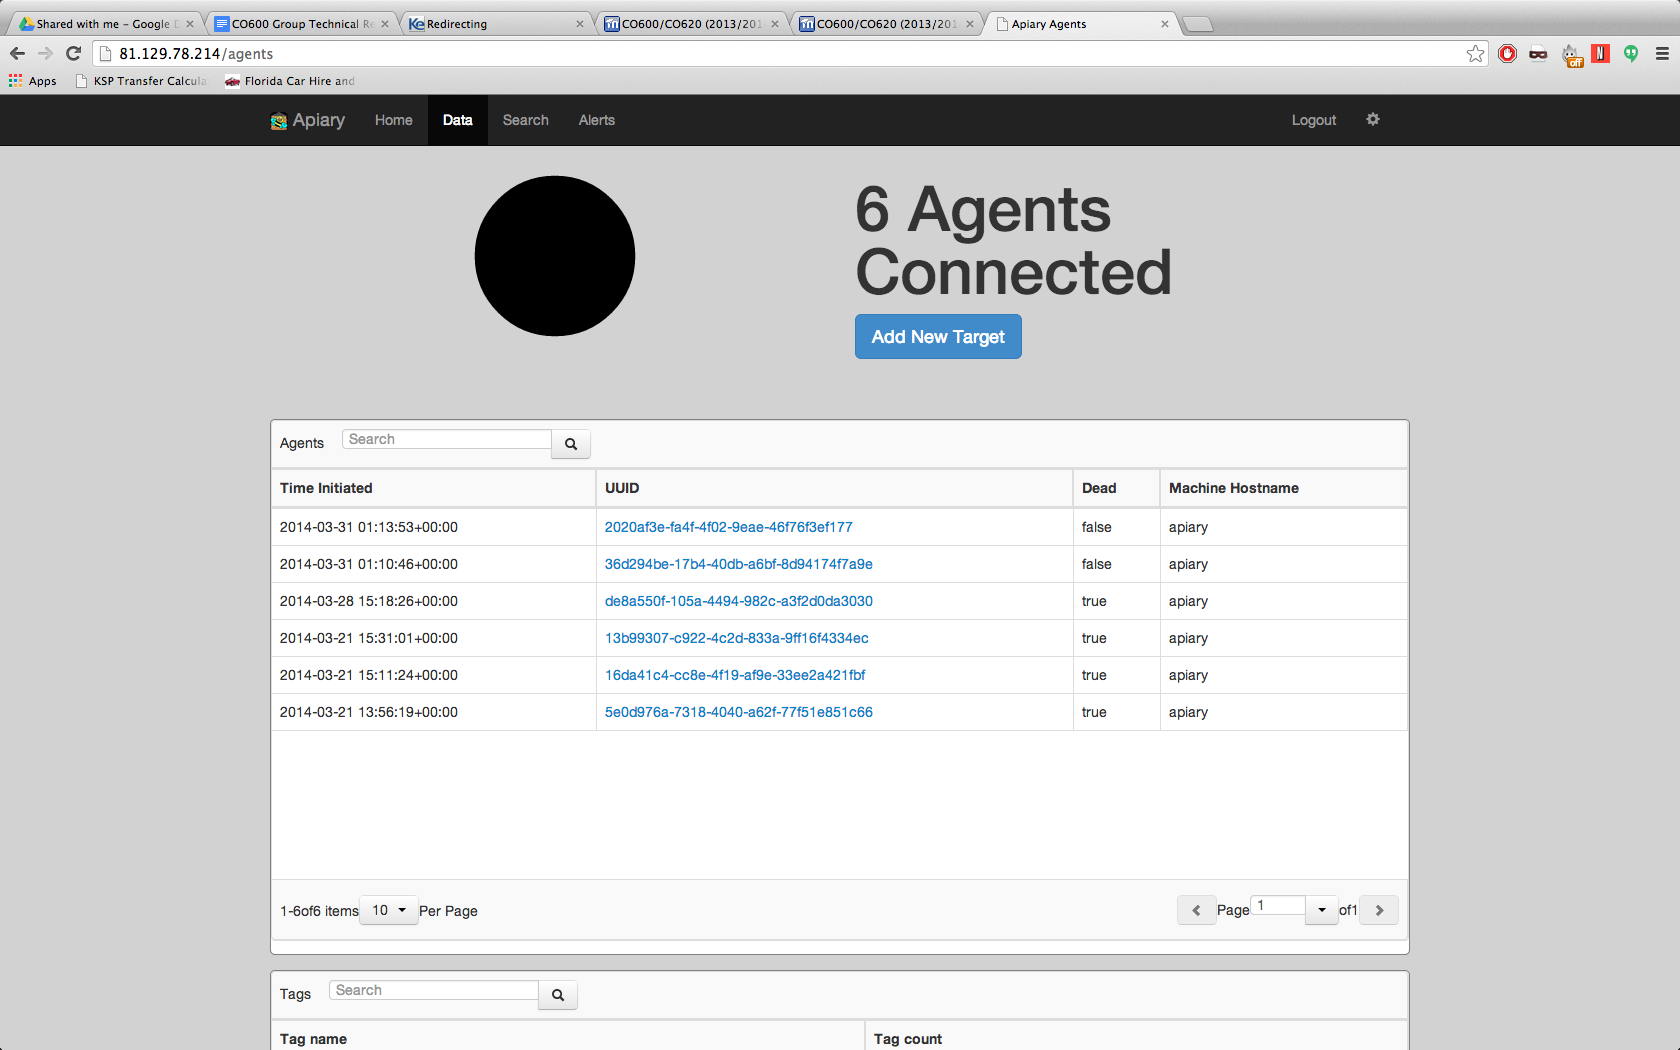
\includegraphics[width=8cm, keepaspectratio]{data.png}
  \caption{Capture of Queens Data page}
\end{figure}

Like the rest of our components Queen uses RabbitMQ for inter-component
communication. The flow for communication with other components is described here
using a user performing a search as an example:

\begin{enumerate}
  \item The search terms are passed from the UI as a JSON object back to Queens
  server via a web-socket.
  \item Queen server then passes this data onto the appropriate Hive component
  via RabbitMQ, using either a remote procedure call or publish/subscribe model
  as appropriate.
  \item The Hive component (in this case Honeycomb) will then return the data to
  Queen server.
  \item The exact data that is required for the front-end is extracted and
  passed back up to the UI via a web-socket.
\end{enumerate}

If we request data using a publish/subscribe model, then every time the Queen
server receives data on the subscribe queue it can push that data back up to the
front-end using a web-socket. This means that the UI always has quick, live
access to the data making our UI responsive, and real time.

Queen enables multiple users to all be using the service at once, so that users
can store and retrieve queries and alerts that the user wants to access next
time they use the system. Also a list of devices associated to the user is
stored for our Alerts system. As with other components MongoDB is used as our
database for this information.

Just as we did with the Bee agents we wanted to keep Queen configuration as
simple as we could. The configuration options as such are kept to just the IP
address of the RabbitMQ server, and the IP address of the mongo server.

Rich visualisations were another key goal in designing Queen, due to our
experience using the d3js\cite{d3} visualisation library we naturally decided to use
this. It has enabled us to use visualisations such as sparkline graphs to map
event rates in the system and pie charts to compare search results. From a human
computer interaction (HCI) point of view this allows the user to process their
data in a much richer format, allowing them to make valuable and meaningful
analysis.

\graphicspath{{./pics/}}
\begin{figure}[h1]
  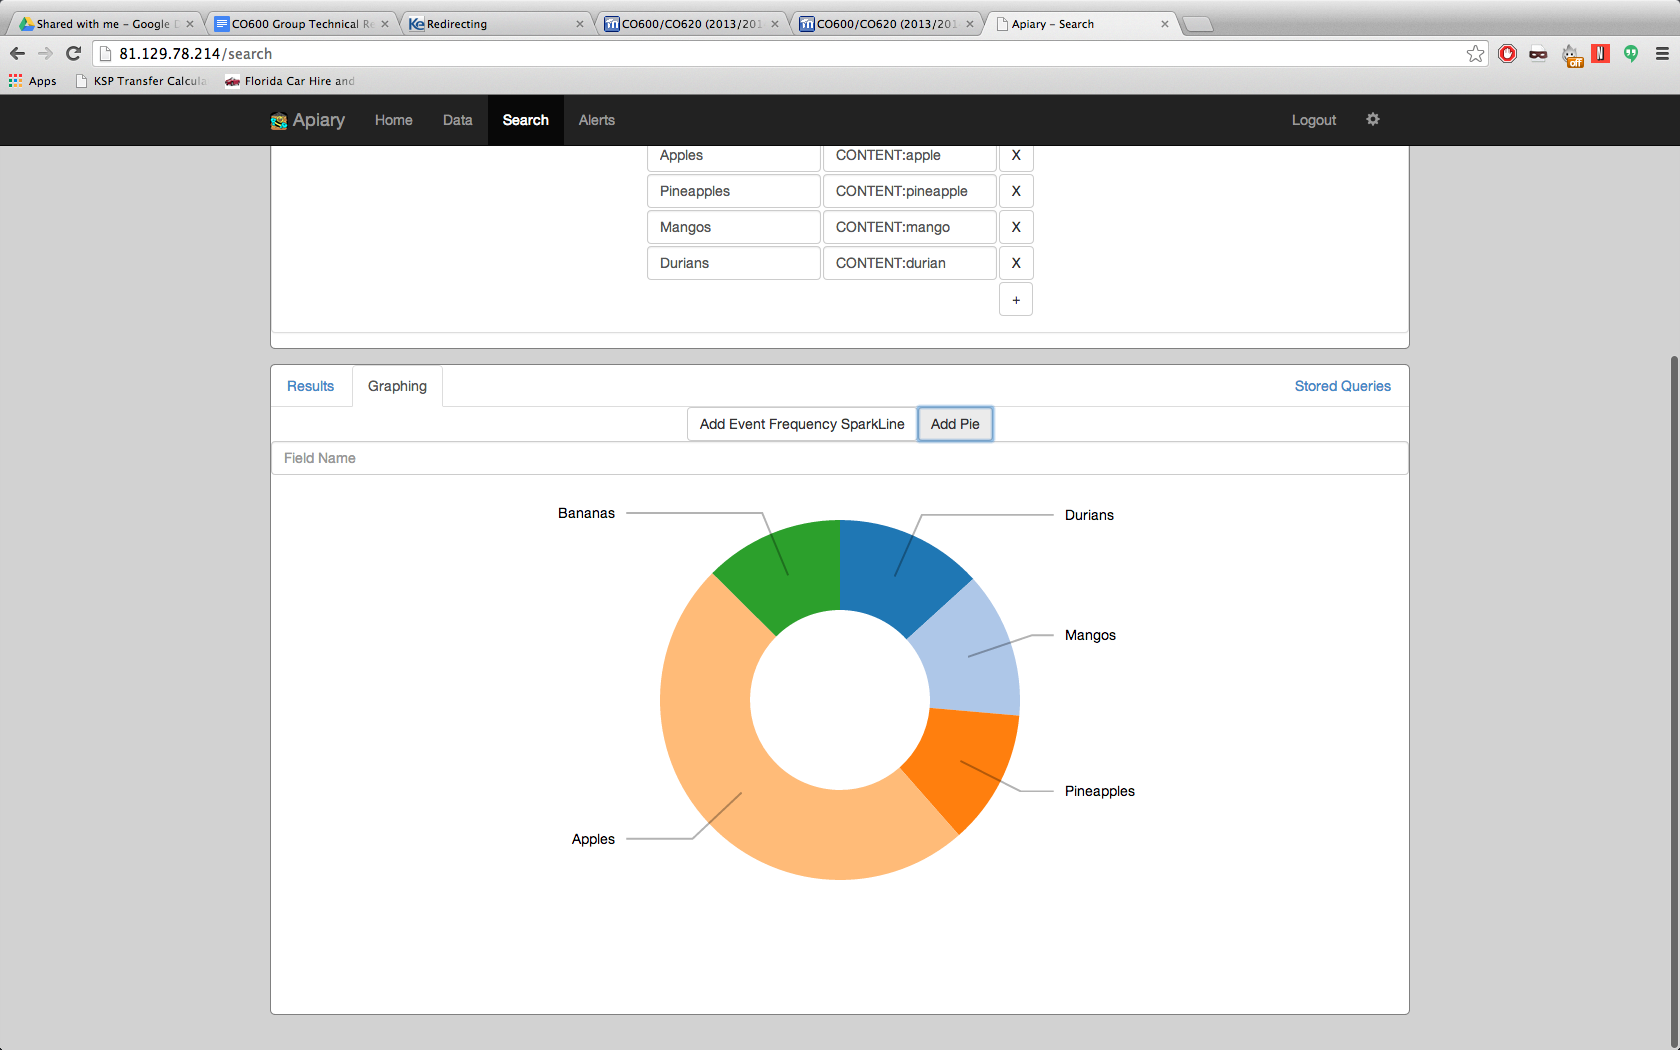
\includegraphics[width=8cm, keepaspectratio]{search.png}
  \caption{Capture of Queens Search page}
\end{figure}

Key to being able to graph data, was being able to infer schema onto our logs
and break queries down into fields. For this we came up with a system whereby a
query could be broken into subqueries, and each of these subqueries could
represent a member of a field. This allowed us to then take the results,
partition them, and graph the various members against one another. The
subqueries are made independently, and the results collated and returned to the
browser. This is what allows us to really gain value from otherwise unorganised
log data, as you can now start to make meaningful analysis.

Due to the quantity of data that can come back from search results it was
important not only to visualise this in graph form but also allow users to view
the actual log entries live in the browser. In order to do this we feed all data
results into a datagrid from the FuelUX\cite{fuelux} library which provides paginated
in-browser tables with column sorting.
